\chapter{Simulations}
\label{ch:simulations}

\section{Overview}
\label{sec:sim_overview}

This chapter presents the Simulink simulations used to evaluate the FWR and NVC topologies of Chapter \ref{ch:topologies}, following the star/delta and anti-series configurations introduced in Sections \ref{sec:fwr} and \ref{sec:nvc}. Before going through each configuration individually, this section describes how the simulations are run and, in particular, how the phase sources and the load are parametrised so that the simulated circuit matches the real prototype as closely as possible.

The real quantities used for this purpose, the phase peak voltages and the current-sensing series resistance described below, come from preliminary measurements taken specifically to support these simulations, not from the full experimental characterisation of the prototype. The complete measurement setup and the actual validation measurements are presented later, in Chapter \ref{ch:measurement_setup}.

The phase model of \eqref{eq:phase_voltage} assumes an ideal sinusoidal EMF of amplitude $E_{pk}$ for every phase, but the voltage actually measured on the prototype is not a perfect sinusoid. Driving the simulation directly with the peak voltage of the real waveform would therefore not reproduce the same power as the real system, since a non-sinusoidal waveform and an ideal sinusoid sharing the same peak value do not, in general, have the same RMS value. For this reason, the peak voltage of each of the six phases was measured directly on the prototype at seven rotational speeds spanning the target range ($100,150,200,250,300,350,400\ \text{rpm}$), giving a $6\times7$ table of real peak voltages $V_\text{pk,real}$, one per phase and speed. The peak voltage of a given phase is not constant from one revolution of the harvester to the next, so $V_\text{pk,real}$ is taken as the average of the peak voltage measured over 100 revolutions at that speed. Since the acquired waveform is a sequence of discrete samples rather than a continuous signal, the RMS value of each measured waveform was computed from the discretised version of its standard definition,
\begin{equation}
    V_\text{rms} \;=\; \sqrt{\frac{1}{N}\sum_{n=1}^{N} v[n]^2},
    \label{eq:rms_def}
\end{equation}
where $v[n]$ are the $N$ samples acquired over multiple full periods of the waveform, corresponding to 100 revolutions. This made it possible to compute a crest factor $\text{CF}\approx1.51$ as the ratio between the peak and the RMS value of the measured waveforms, close to but slightly above the value $\sqrt{2}\approx1.414$ that an ideal sinusoid would give, reflecting the fact that the real EMF is not perfectly sinusoidal. Since $\text{CF}>\sqrt{2}$, this implies that, at the same peak value, the real EMF delivers less power than an ideal sinusoidal waveform.

Figures \ref{fig:ocv_half} and \ref{fig:ocv_focus} show, as a representative example, the open-circuit voltage measured on all six phases at $100\ \text{rpm}$. Figure \ref{fig:ocv_half} covers half a revolution of the harvester and shows the general shape of the measured waveform, visibly different from ideal sinusoids. Figure \ref{fig:ocv_focus} focuses on a short time window to highlight the $60^\circ$ phase shift between consecutive phases. The peak-to-peak voltage is not identical across the six phases: this is not a measurement artefact, but a consequence of manufacturing tolerances between the six nominally identical pickup units of the prototype, which is also why each phase is treated individually in Table \ref{tab:sim_voltage} rather than assumed identical.

\begin{figure}[h!]
    \centering
    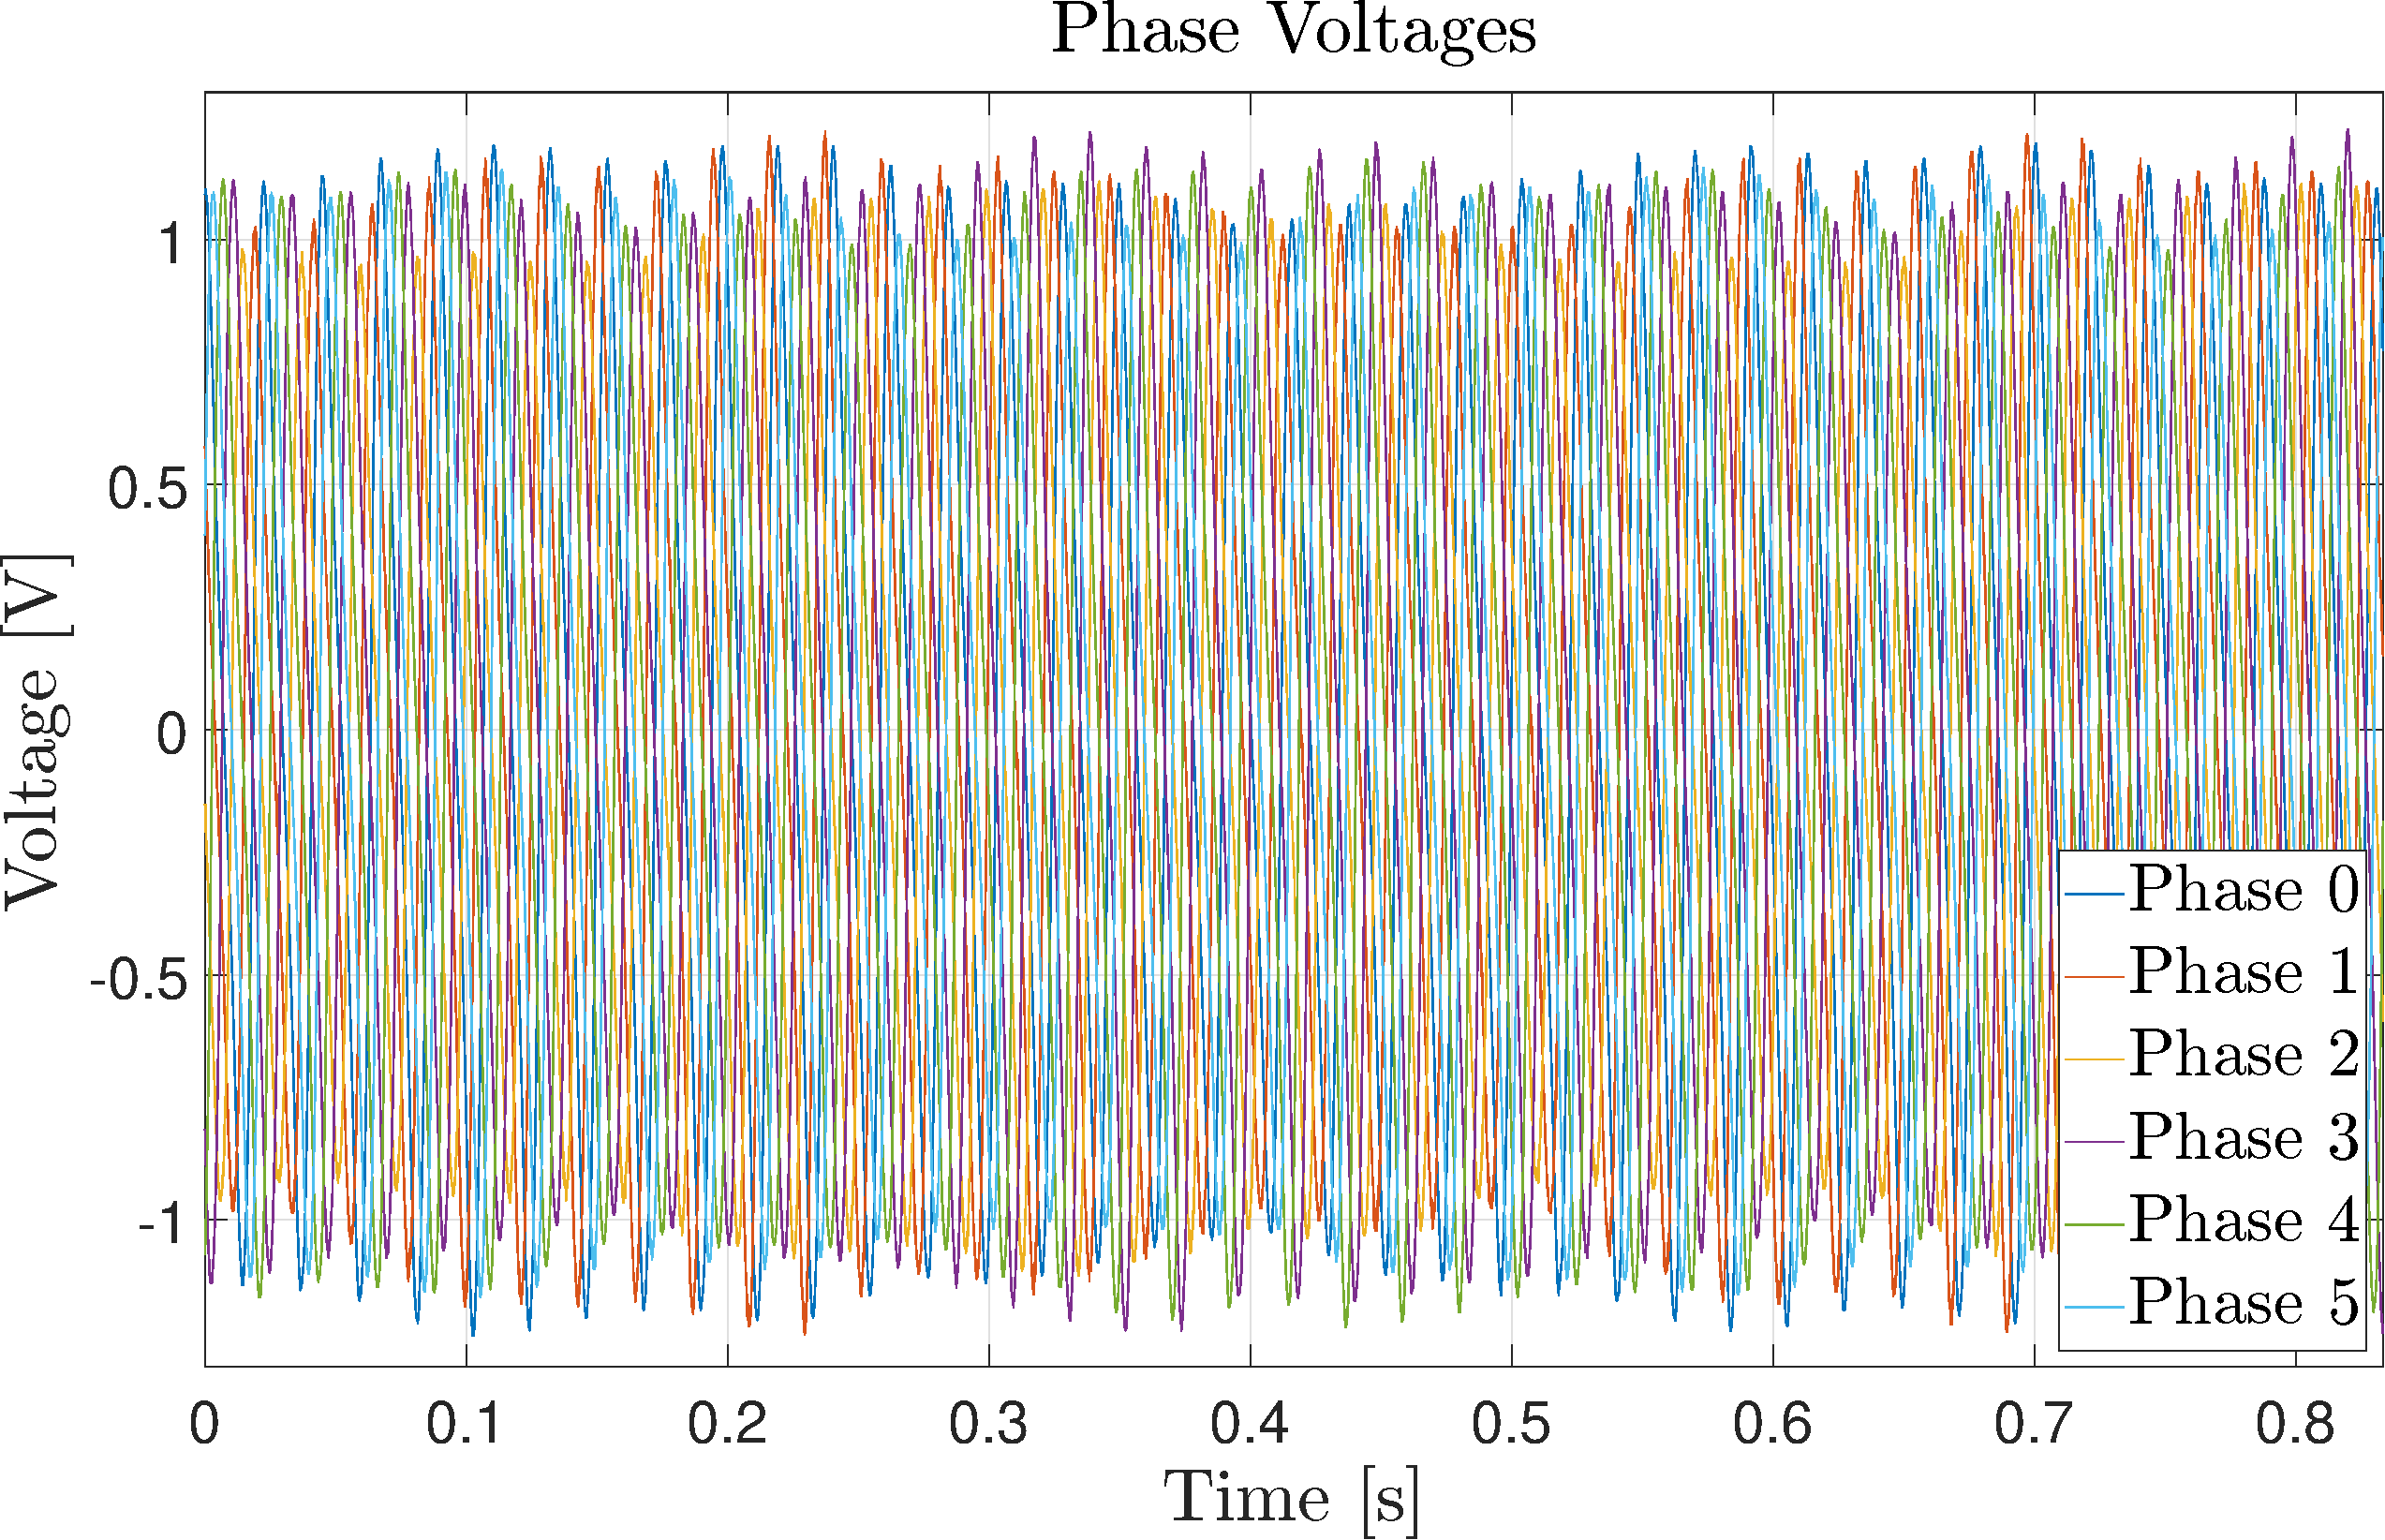
\includegraphics[width=0.85\textwidth]{Plots/OCV_100_halfTourn.pdf}
    \caption{Open-circuit voltage measured on all six phases over half a revolution of the harvester at $100\ \text{rpm}$.}
    \label{fig:ocv_half}
\end{figure}

\begin{figure}[h!]
    \centering
    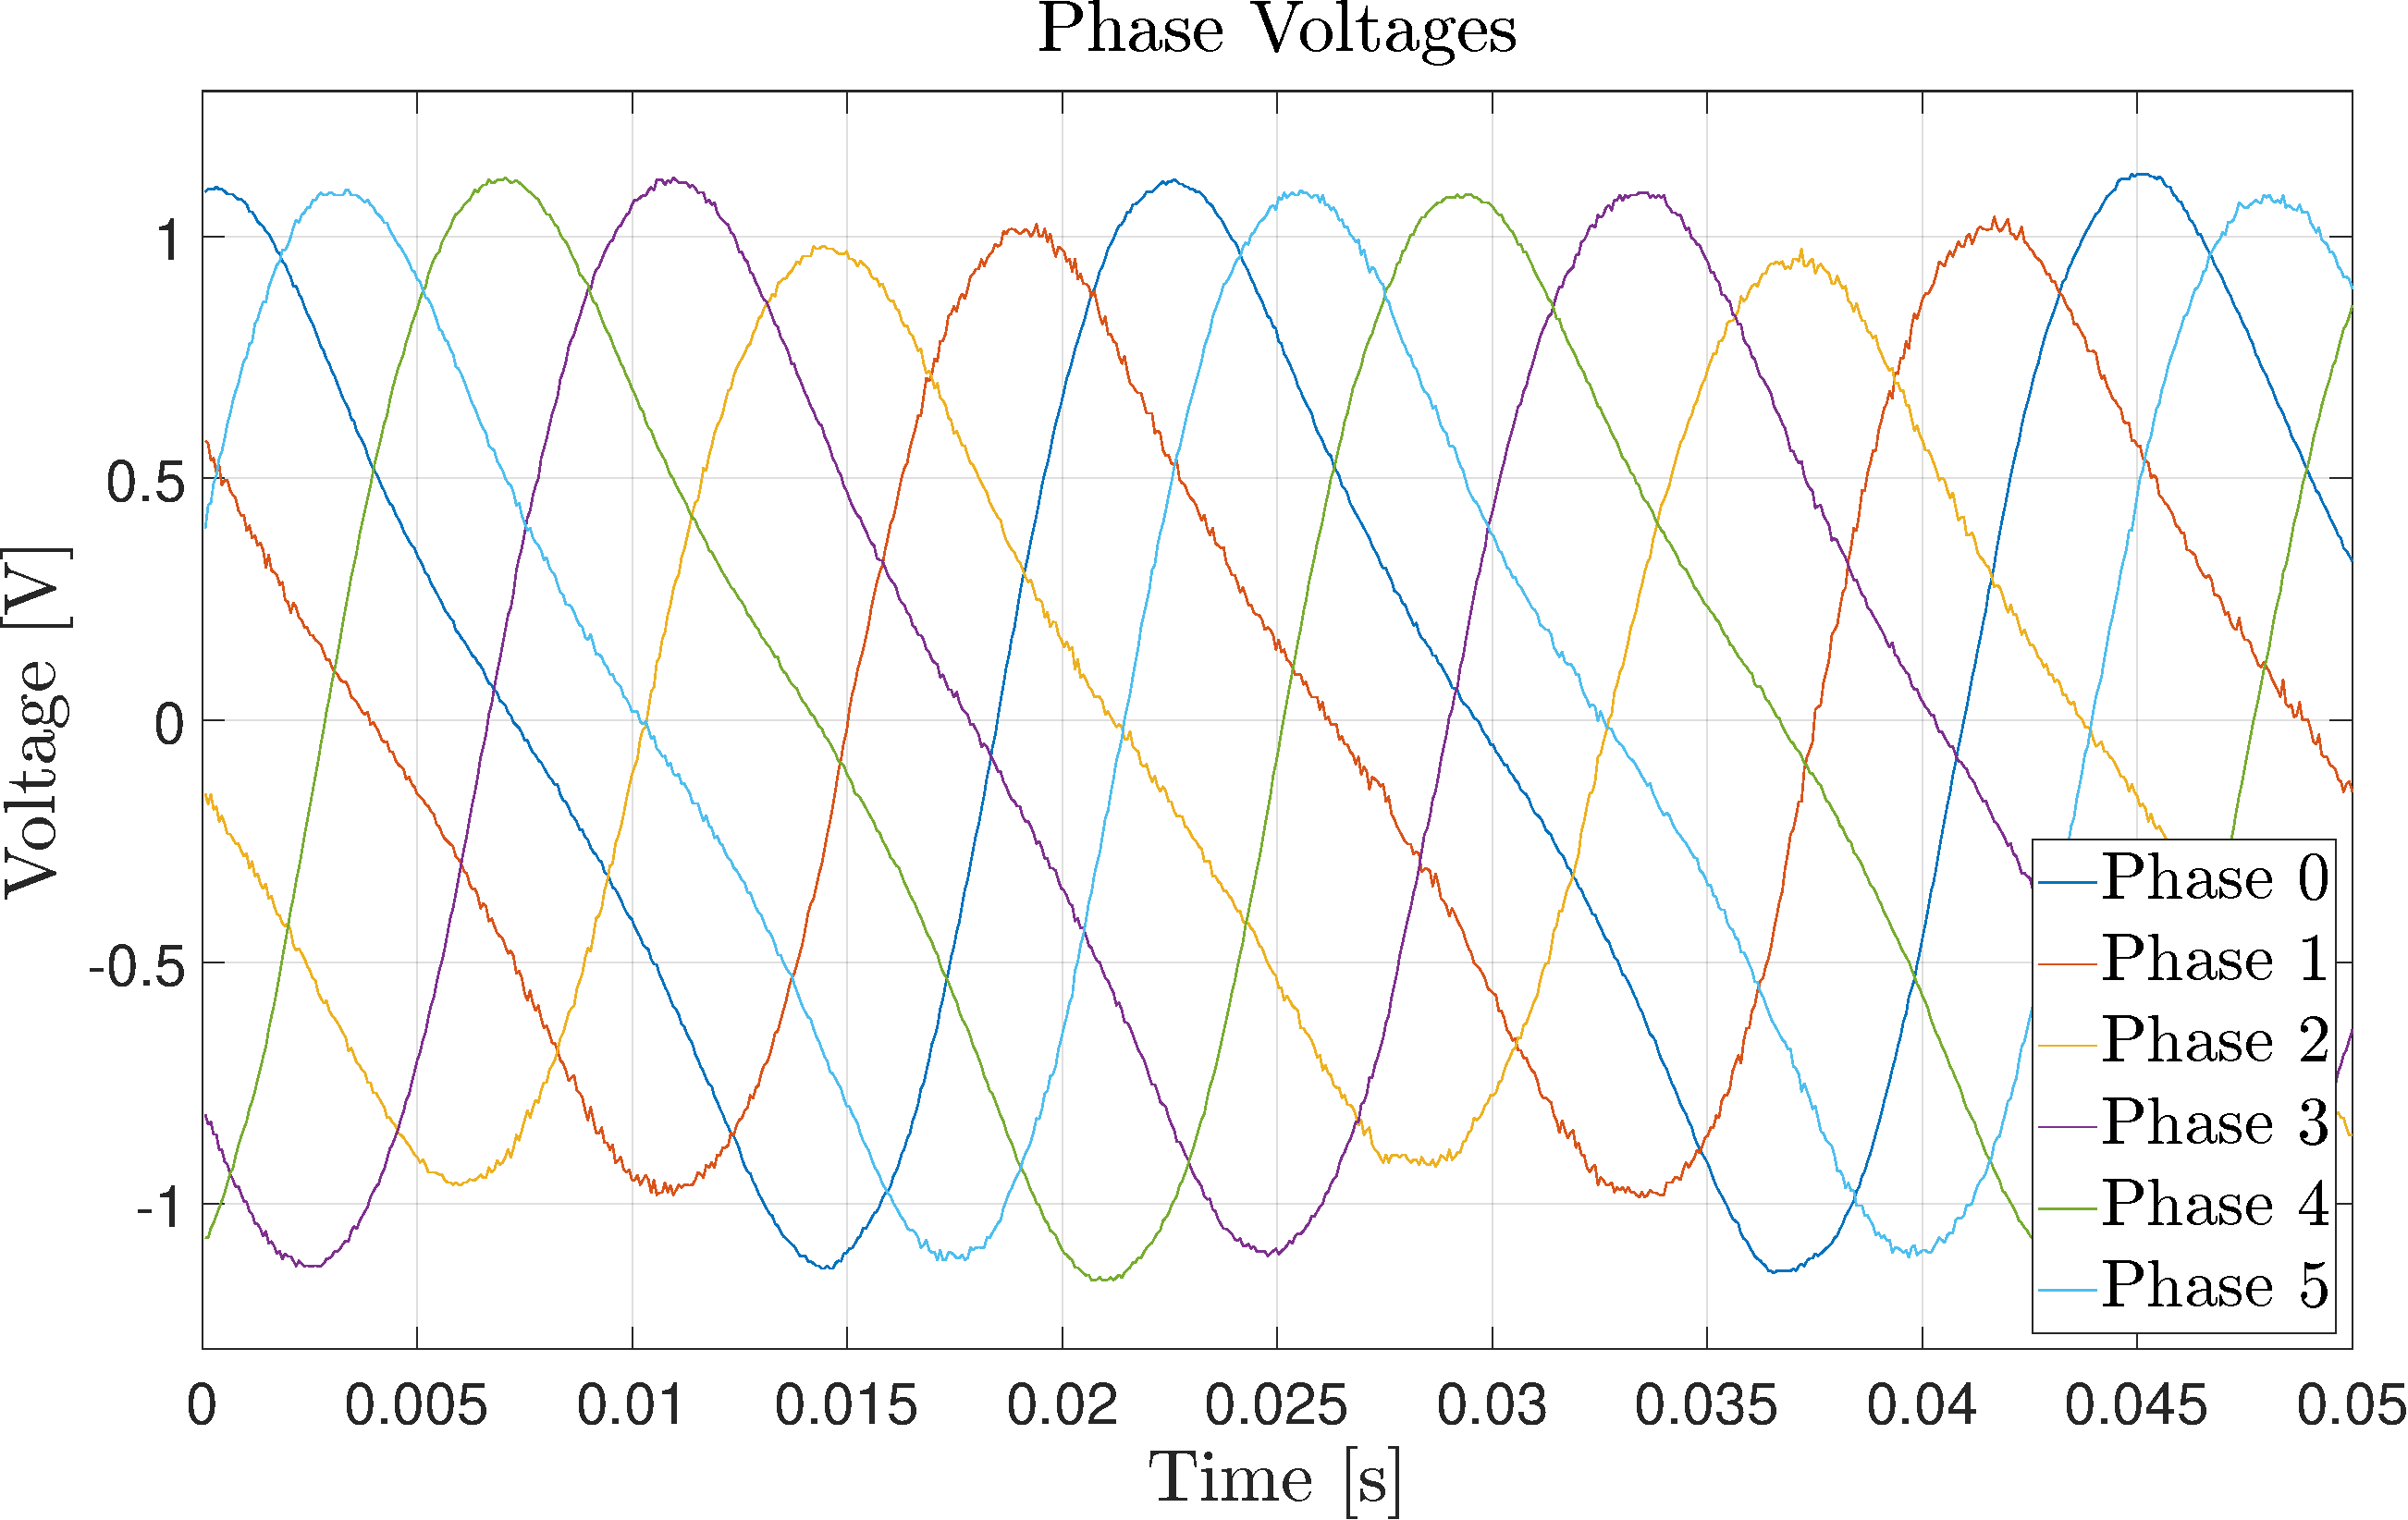
\includegraphics[width=0.85\textwidth]{Plots/OCV_100_focus.pdf}
    \caption{Detail of the same measurement, showing the $60^\circ$ phase shift between the six phase voltages.}
    \label{fig:ocv_focus}
\end{figure}

Each phase is still represented in the Simulink model as an ideal sinusoidal source, consistently with \eqref{eq:phase_voltage}, but rather than using $V_\text{pk,real}$ directly as its amplitude, every tabulated value is rescaled by $\sqrt{2}/\text{CF}$,
\begin{equation}
    V_s \;=\; V_\text{pk,real}\cdot\frac{\sqrt{2}}{\text{CF}} \;=\; \sqrt{2}\,V_\text{rms,real},
    \label{eq:sim_voltage_scaling}
\end{equation}
for every phase and every simulated speed, since $\text{CF}$ is, by definition, the ratio of the real peak to the real RMS value. $V_s$ is therefore the peak of the ideal sinusoid whose RMS value, and therefore whose power, equals that of the real measured phase voltage.

Table \ref{tab:sim_voltage} lists the resulting value of $V_s$ used for each of the six coils at each of the seven simulated speeds.

\begin{table}[htbp]
    \centering

    \begin{tabular}{cccccccc}
        \toprule
        & \multicolumn{7}{c}{Rotational speed (rpm)} \\
        \cmidrule(lr){2-8}
        Coil & 100 & 150 & 200 & 250 & 300 & 350 & 400 \\
        \midrule
        0 & 1.055 & 1.480 & 1.913 & 2.326 & 2.744 & 3.179 & 3.601 \\
        1 & 1.041 & 1.458 & 1.862 & 2.255 & 2.652 & 3.036 & 3.344 \\
        2 & 0.964 & 1.352 & 1.722 & 2.092 & 2.464 & 2.847 & 3.239 \\
        3 & 1.052 & 1.463 & 1.872 & 2.288 & 2.712 & 3.128 & 3.542 \\
        4 & 1.020 & 1.418 & 1.815 & 2.230 & 2.627 & 3.030 & 3.349 \\
        5 & 0.997 & 1.393 & 1.803 & 2.197 & 2.592 & 3.006 & 3.408 \\
        \bottomrule
    \end{tabular}
    \caption{Equivalent sinusoidal peak voltage $V_s$ (V) used for each of the six coils in the Simulink simulations, computed from \eqref{eq:sim_voltage_scaling}.}
    \label{tab:sim_voltage}
\end{table}

Figure \ref{fig:voltage_comp} illustrates this correction for phase 0 (coil 0) across the whole target speed range, comparing three quantities: the peak voltage predicted by the finite-element (COMSOL) model behind the reference parameters of Table \ref{tab:vreh_par}, the raw measured peak voltage $V_\text{pk,real}$ used directly as if the phase were an ideal sinusoid, and the crest-factor-corrected equivalent sinusoidal voltage $V_s$ of \eqref{eq:sim_voltage_scaling}. At the low-speed end of the range, both the raw and the crest-factor-corrected voltage remain well below the FEM prediction, and the correction changes a little. Moving towards the high-speed end, both curves rise past the FEM prediction, but the raw measurement crosses it earlier, around $340\ \text{rpm}$, and overshoots it the most by $400\ \text{rpm}$; the crest-factor correction delays this crossing to near the end of the range and leaves a much smaller gap at $400\ \text{rpm}$, bringing the corrected voltage into closer agreement with the FEM prediction. As already noted, the real voltage is lower than the FEM prediction for most of the speed range, so the power it corresponds to is lower too.

\begin{figure}[h!]
    \centering
    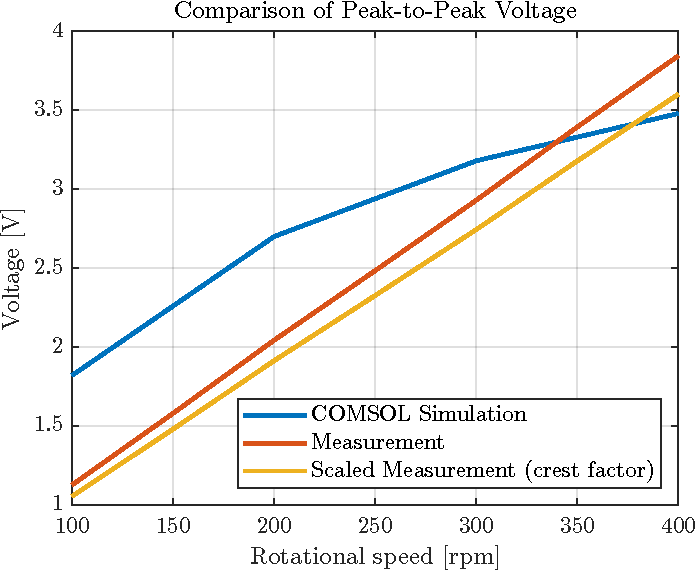
\includegraphics[width=0.75\textwidth]{Plots/Voltage_comp.pdf}
    \caption{Peak voltage of phase 0 across the target speed range: the COMSOL finite-element prediction, the raw measured value used directly as an idealised sinusoid, and the same value corrected by the crest factor.}
    \label{fig:voltage_comp}
\end{figure}

The simulated circuit also accounts for the current-sensing system used in the experimental setup of Chapter \ref{ch:measurement_setup}. The shunt resistor, the INA114AU sensing board and the connecting cables together introduce a series resistance that is not part of the idealised topologies; measured directly, this resistance is approximately $1.5\ \Omega$. Since this value is not negligible compared to the coil resistance $R_\text{Coil} = 6\ \Omega$ of Table \ref{tab:vreh_par}, it is included in the Simulink model as an additional series resistance in the same branch as each coil and in the branch feeding the load, so that the simulated circuit is loaded in the same way as the real prototype during the measurements.


\section{Full-Wave Rectifier (FWR)}
\label{sec:sim_fwr}

\subsection{Star Connection}
\label{sec:sim_fwr_star}

\subsubsection{First Bridge (FWR1, $k=0,2,4$)}
\label{sec:sim_fwr1_star}

\subsubsection{Second Bridge (FWR2, $k=1,3,5$)}
\label{sec:sim_fwr2_star}

\subsubsection{Both Bridges}
\label{sec:sim_fwr_star_both}

\subsection{Delta Connection}
\label{sec:sim_fwr_delta}

\subsubsection{First Bridge (FWR1, $k=0,2,4$)}
\label{sec:sim_fwr1_delta}

\subsubsection{Second Bridge (FWR2, $k=1,3,5$)}
\label{sec:sim_fwr2_delta}

\subsubsection{Both Bridges}
\label{sec:sim_fwr_delta_both}

\section{Negative Voltage Converter (NVC)}
\label{sec:sim_nvc}

\subsection{First Bridge (NVC1, $k=0,3$)}
\label{sec:sim_nvc1}

\subsection{Second Bridge (NVC2, $k=1,4$)}
\label{sec:sim_nvc2}

\subsection{Third Bridge (NVC3, $k=2,5$)}
\label{sec:sim_nvc3}

\subsection{All Three Bridges}
\label{sec:sim_nvc_all}
